% This is the template Jun uses for project seeds
% jun.allard@uci.edu allardlab.com
\documentclass[onecolumn,11pt]{article}

% --------- required packages ---------
\usepackage{enumerate}
\usepackage{enumitem}
\usepackage{graphicx}
\usepackage[colorlinks,allcolors=black]{hyperref}
\usepackage[font=small]{caption}
\usepackage{siunitx}
\usepackage{times}
\usepackage{titlesec}

\usepackage{titling}
\usepackage{authblk} % must come after titling package loading

% --------- standard packages ---------
%\usepackage{amsfonts}
\usepackage{amsmath}
\usepackage{amssymb}
%\usepackage{array}
%\usepackage{bm}
%\usepackage{color}
%\usepackage{chemarr}
%\usepackage{float}
\usepackage[utf8]{inputenc}
\usepackage{lipsum}
%\usepackage{mathtools}
%\usepackage{multicol}
%\usepackage{multirow}
%\usepackage{pdfsync}
%\usepackage{tocloft}
%\usepackage{verbatim}
%\usepackage{wrapfig}


% --------- packages, less often used ---------
%\usepackage[export]{adjustbox}
%\usepackage{amsopn}
%\usepackage{cancel} % adds strikethrough
%\usepackage{CJK} % Chinese Japanese Korean
%\usepackage{dcolumn} % align columns in a table
%\usepackage{dsfont}
%\usepackage{epsfig}
%\usepackage{epstopdf}
%\usepackage{esint} % integrals
%\usepackage{framed}
%\usepackage{physics} %for \vqty, \dd, \dv
%\usepackage{rotating}
%\usepackage{setspace} % set space between lines
%\usepackage{subcaption}
%\usepackage{tcolorbox}
%\usepackage[normalem]{ulem} % for underlining
% --------- for typesetting code blocks --------
%\usepackage{algorithmic} % for code including Matlab
%\usepackage{listings} % for code including Matlab
%\usepackage[numbered,framed,basicstyle]{matlab-prettifier}




\usepackage{internalsubfigures}




%%%%%%%%%%%%%%%%%%%%%%%%%%%%%%%%%%%%%%%%%%%%%%%%%%%%%%%%%%%%
% page layout
\usepackage[margin=1in]{geometry}

% paragraph layout
\setlength{\parindent}{0pt} % paragraph indent - looks best zero
\setlength{\parskip}{0.8em plus 0.1em minus 0.1em} % paragraph spacing
\setlist[itemize]{itemsep=0.0em,topsep=0em}
\setlist[enumerate]{itemsep=0.0em,topsep=0em}
\titlespacing{\paragraph}{0em}{-0.8em}{1em} % for the /paragraph command

% Bibliography setup
\usepackage[numbers,square,sort&compress]{natbib}
\bibliographystyle{unsrtnat}
%\bibliographystyle{biophysj}

\title{Project JeanJacket}
\author[a]{Jun}
\affil[a]{University of California Irvine}


%%%%%%%%%%%%%%%%%%%%%%%%%%%%%%%%%%%%%%%%%%%%%%%%%%%%%%%
\date{} % leave blank for no date
\begin{document}

\maketitle
%%%%%%%%%%%%%%%%%%%%%%%%%%%%%%%%%%%%%%%%%%%%%%%%%%%%%%%

%\begin{abstract}
%Nothing here yet
%\end{abstract}


% \internalsubfigure{appleref}{Apple}
% \internalsubfigure{orangeref}{Orange}
% \internalsubfigure{zucchinniref}{Zucchinni}

%\processinternalcaption

% \begin{myenvironment}

%         \appendtomylist{appleref}{An apple. }
%         \appendtomylist{zucchiniref}{A zucchinni. }

%         % The environment can use \mylist here, which has accumulated content.
% \end{myenvironment}


\clearpage


\begin{figure}[ht]
        \centering
        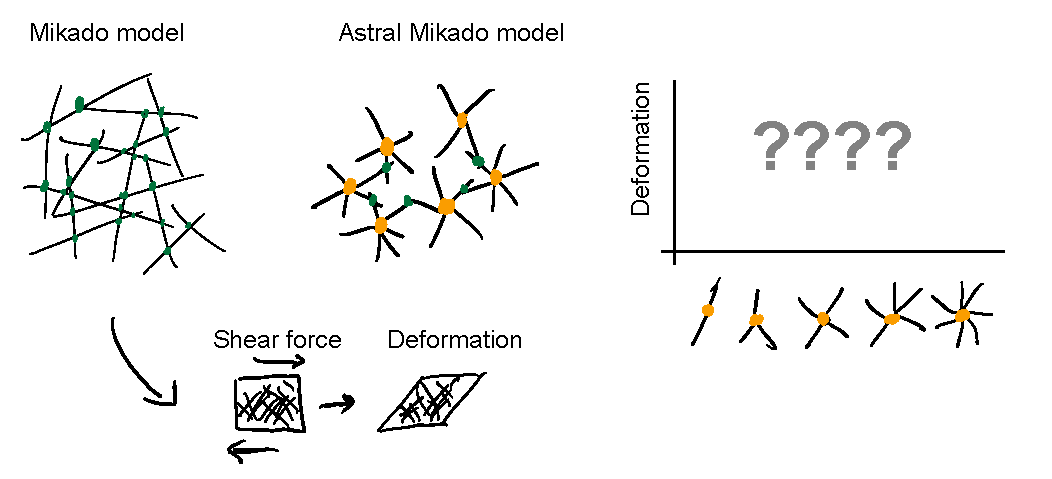
\includegraphics[width=4.5in]{figures/figJeanJacket.pdf}
        \begin{internalcaption}
                %\processmylist
                \internalsubfigure{fig:track}{(A) A track that means nothing on its own}
                \internalsubfigure{fig:pcolor}{(B) A pcolor map that also means nothing on its own}
        \end{internalcaption}
        %\label{fig:omics_conclusion}
\end{figure}



I would like to refer to the main figure Figure~\ref{fig:omics_conclusion}. But this less informative, and instead I should refer to specific panels.

Now, I would like to just refer to the track, Figure~\ref{fig:track}.

Now, I would like to just refer to the colormap, Figure~\ref{fig:pcolor}.



\clearpage




\begin{figure}[ht]
        \centering
        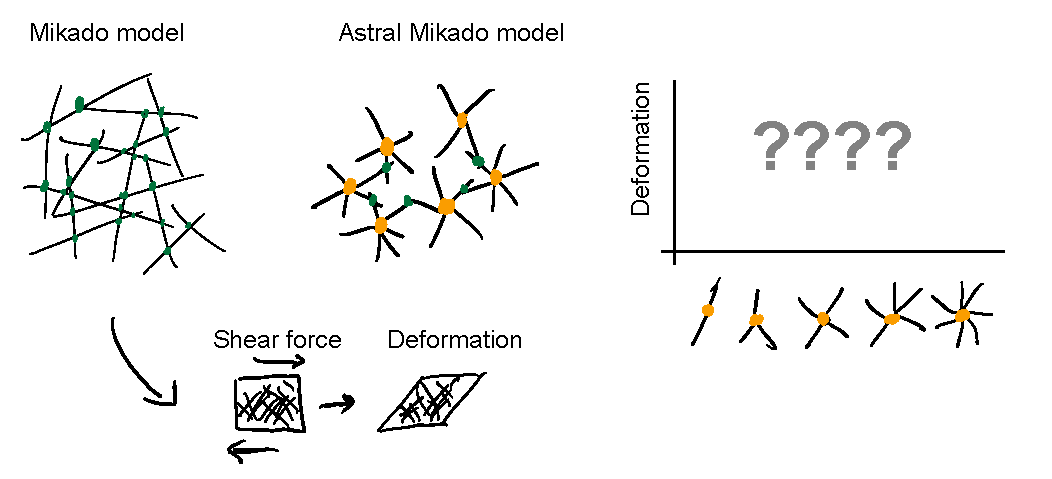
\includegraphics[width=4.5in]{figures/figJeanJacket.pdf}

        \internalsubfigurelabel{fig:gel}
        \internalsubfigurelabel{fig:heatmap}

        \caption{A huge figure with a billion subfigures. 
        (A) a gel that means something profound. 
        (B) a heatmap that explains everything.}
        \label{fig:main_conclusion}
\end{figure}
    

I would like to refer to the main figure Figure~\ref{fig:main_conclusion}. But this less informative, and instead I should refer to specific panels.

Now, I would like to just refer to the gel, Figure~\ref{fig:gel}.

Now, I would like to just refer to the heatmap, Figure~\ref{fig:heatmap}.




% \newpage
% \begin{figure}[ht]
%         \centering
%         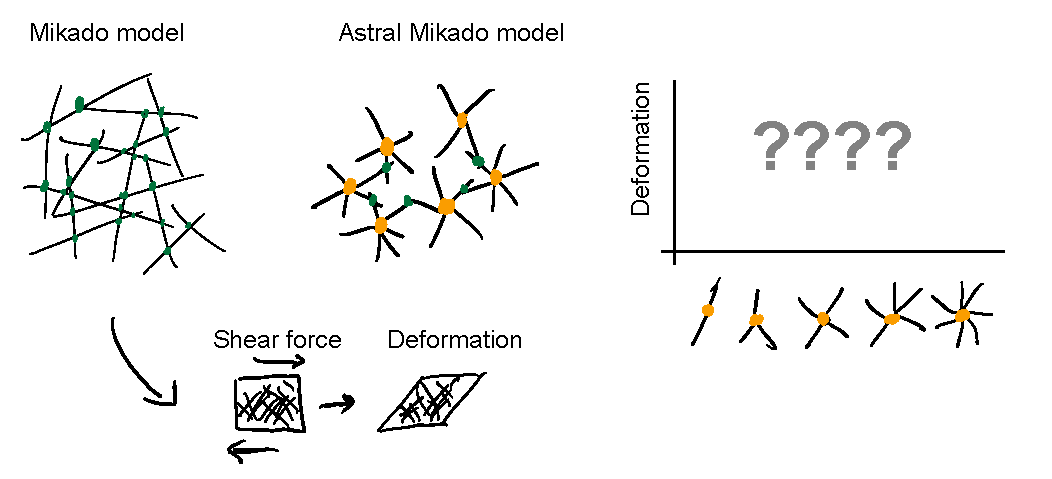
\includegraphics[width=4.5in]{figures/figJeanJacket.pdf}
%         \internalsubfigurelabel{fig:schematic}
%         \internalsubfigurelabel{fig:refereeexperiment}
%         \caption{A huge figure with a billion subfigures. 
%         (A) a schematic that shows the parts of the project. 
%         (B) a stupid experiment requested by Referee \#3.}
%         \label{fig:secondaryconclusion}
% \end{figure}

% I would like to refer to the main secondary figure Figure~\ref{fig:secondaryconclusion}.

% Now, I would like to just refer to the schematic, Figure~\ref{fig:schematic}.

% Now, I would like to just refer to the referee experiment, Figure~\ref{fig:refereeexperiment}.



\end{document}

